\documentclass[a4paper,12pt]{article}
\usepackage[top = 2.5cm, bottom = 2.5cm, left = 2.5cm, right = 2.5cm]{geometry}
\usepackage[T1]{fontenc}
\usepackage[utf8]{inputenc}
\usepackage{multirow} 
\usepackage{booktabs} 
\usepackage{graphicx}
\usepackage[spanish]{babel}
\usepackage{setspace}
\setlength{\parindent}{0in}
\usepackage{float}
\usepackage{fancyhdr}
\usepackage{amsmath}
\usepackage{amssymb}
\usepackage{amsthm}
\usepackage[numbers]{natbib}
\newcommand\Mycite[1]{%
	\citeauthor{#1}~[\citeyear{#1}]}
\usepackage{graphicx}
\usepackage{subcaption}
\usepackage{booktabs}
\usepackage{etoolbox}
\usepackage{minibox}
\usepackage{hyperref}
\usepackage{xcolor}
\usepackage[skins]{tcolorbox}
%---------------------------

\newtcolorbox{cajita}[1][]{
	 #1
}

\newenvironment{sol}
{\renewcommand\qedsymbol{$\square$}\begin{proof}[\textbf{Solución.}]}
	{\end{proof}}

\newenvironment{dem}
{\renewcommand\qedsymbol{$\blacksquare$}\begin{proof}[\textbf{Demostración.}]}
	{\end{proof}}

\newtheorem{problema}{Problema}
\newtheorem{definicion}{Definición}
\newtheorem{ejemplo}{Ejemplo}
\newtheorem{teorema}{Teorema}
\newtheorem{corolario}{Corolario}[teorema]
\newtheorem{lema}[teorema]{Lema}
\newtheorem{prop}{Proposición}
\newtheorem*{nota}{\textbf{NOTA}}
\renewcommand\qedsymbol{$\blacksquare$}
\usepackage{svg}
\usepackage{tikz}
\usepackage[framemethod=default]{mdframed}
\global\mdfdefinestyle{exampledefault}{%
linecolor=lightgray,linewidth=1pt,%
leftmargin=1cm,rightmargin=1cm,
}




\newenvironment{noter}[1]{%
\mdfsetup{%
frametitle={\tikz\node[fill=white,rectangle,inner sep=0pt,outer sep=0pt]{#1};},
frametitleaboveskip=-0.5\ht\strutbox,
frametitlealignment=\raggedright
}%
\begin{mdframed}[style=exampledefault]
}{\end{mdframed}}
\newcommand{\linea}{\noindent\rule{\textwidth}{3pt}}
\newcommand{\linita}{\noindent\rule{\textwidth}{1pt}}

\AtBeginEnvironment{align}{\setcounter{equation}{0}}
\pagestyle{fancy}

\fancyhf{}









%----------------------------------------------------------
\lhead{\footnotesize Álgebra Moderna}
\rhead{\footnotesize  Rudik Roberto Rompich}
\cfoot{\footnotesize \thepage}


%--------------------------

\begin{document}
 \thispagestyle{empty} 
    \begin{tabular}{p{15.5cm}}
    \begin{tabbing}
    \textbf{Universidad del Valle de Guatemala} \\
    Departamento de Matemática\\
    Licenciatura en Matemática Aplicada\\\\
   \textbf{Estudiante:} Rudik Roberto Rompich\\
   \textbf{Correo:}  \href{mailto:rom19857@uvg.edu.gt}{rom19857@uvg.edu.gt}\\
   \textbf{Carné:} 19857
    \end{tabbing}
    \begin{center}
        MM2035 - Álgebra Moderna - Catedrático: Ricardo Barrientos\\
        \today
    \end{center}\\
    \hline
    \\
    \end{tabular} 
    \vspace*{0.3cm} 
    \begin{center} 
    {\Large \bf  Tarea 13
} 
        \vspace{2mm}
    \end{center}
    \vspace{0.4cm}
%--------------------------
Problemas 2, 5, 6, 7, 11, 12 y 13, sección 5.3


\begin{problema}[Problema 2]

In the proof of Theorem 5.3.1, prove in all detail that the elements $1+V, x+V, \ldots, x^{n-1}+V$ form a basis of $E$ over $F$.
\begin{dem}
    \textbf{Detalles del teorema demostrado en clase:}
    \begin{figure}[H]
        \centering
        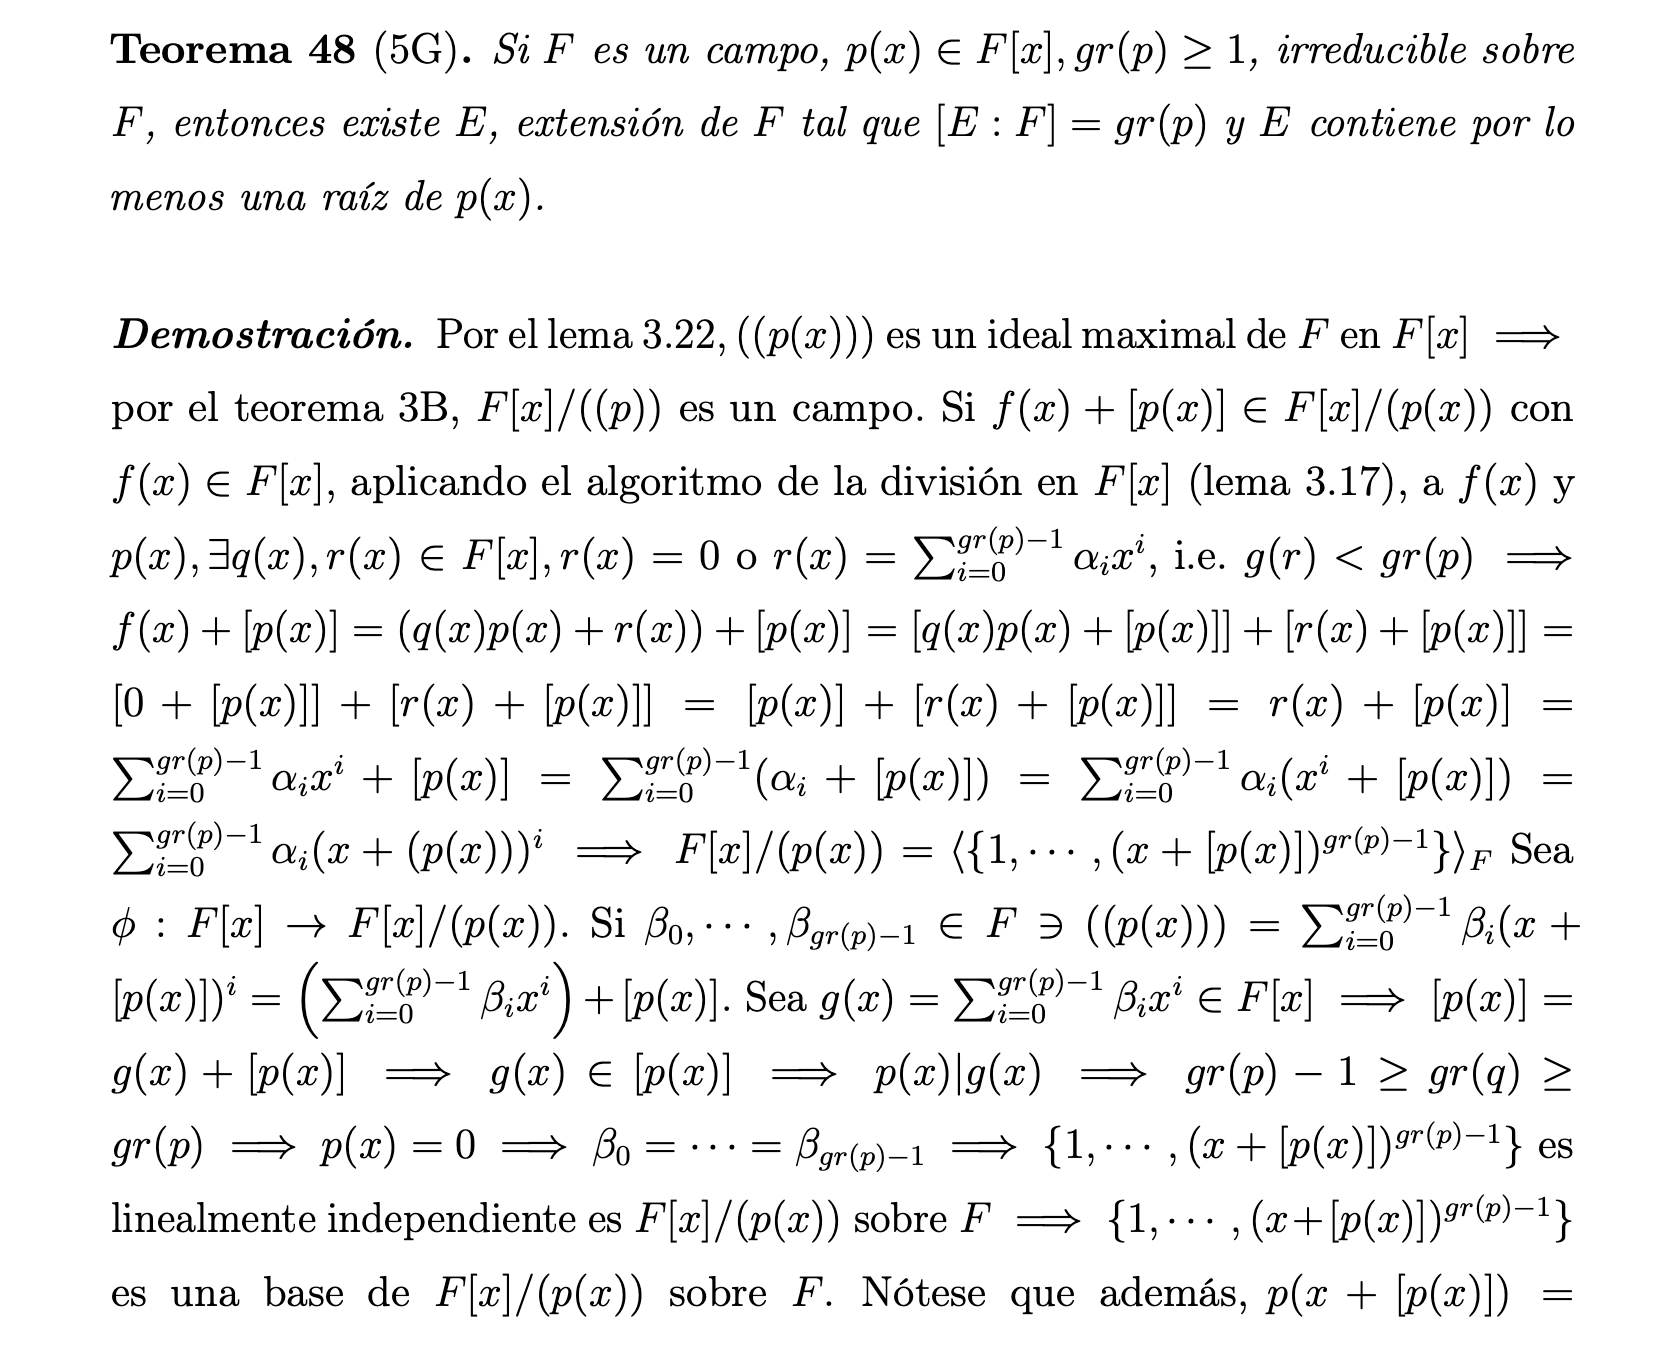
\includegraphics[scale=0.5]{Problemas/dem1.png}
    \end{figure}
\end{dem}
\end{problema}

\begin{problema}[Problema 5]
    In Example 3 at the end of this section prove that $F(\omega)$ is the splitting field of $x^4+x^2+1$.
    \begin{dem}
        Nótese que 
        $$f(x)=x^4+x^2+1 = (x-w)(x+w)(x-w^2)(x+w^2),$$
        tal que $f(x)$ es irreducible sobre $F$ en $F(w)$.
    \end{dem}

\end{problema}

\begin{problema}[Problema 6]
    Let $F$ be the field of rational numbers. Determine the degrees of the splitting fields of the following polynomials over $F$.
    \begin{enumerate}
        \item $x^4+1$.
        \begin{dem}
            Sea 
            $$f(x)=x^4+1=(x-w)(x+w)(x-w^3)(x+w^3),$$
            en donde las raíces son complejas. Entonces $x^4+1$ es irreducible por criterio de Eisenstein. Además su grado es 4. 
        \end{dem}
        \item $x^6+1$.
        \begin{dem}
            Sea 
            $$f(x)=x^6+1=(x-i)(x+i)(x^4+x^2+1)=(x-i)(x+i)(x-w)(x+w)(x-w^2)(x+w^2),$$
            entonces $f(x)$ es irreducible sobre $F(w)$. Además por el \textbf{Problema 2}, sabíamos que $^4+x^2+1$ es irreducible sobre $F$ con grado 4 por Eisenstein. Por lo tanto, $x^6+1$ también es de grado 4. 
        \end{dem}
        \item $x^4-2$.
        \begin{dem}
            Sea
            $$f(x)=x^4-2 = (x-\sqrt[4]{2})(x+\sqrt[4]{2})(x-i\sqrt[4]{2})(x+i\sqrt[4]{2}),$$
            de esto tenemos que el campo de descomposición es $F(\sqrt[4]{2},i)$. Además, nótese que $x^2+1$ es irreducible en $F(\sqrt[4]{2})$ tal que $[F(\sqrt[4]{2},i):F(\sqrt[4]{2})]=2$ y por otra parte, se tiene que $[F(\sqrt[4]{2}):F]=4$. Entonces, el grado es $[F(\sqrt[4]{2},i):F(\sqrt[4]{2})[F(\sqrt[4]{2}):F]]=8$.
        \end{dem}
        \item $x^5-1$.
        \begin{dem}
            Sea
            $$f(x)=x^5-1=(x-w)(x-w^2)(x-w^3)(x-w^4)(x-w^5),$$
            entonces $f(x)$ es irreducible sobre $F(w)$. Por otra parte, nótese que $x^4+x^3+x^2+x+1$ es irreducible en $F$ con grado 4, y por lo tanto $x^5-1$ también tiene grado 4. 
        \end{dem}
        \item $x^6+x^3+1$.
        \begin{dem}
            Sea
            \begin{align*}
                f(x)=x^6+x^3+1 =(x-w)(x+w)(x-w^4)(x+w^4)(x-w^7)(x+w^7),
            \end{align*}
            entonces $f(x)$ es irreducible sobre $F(w)$. Entonces, por Eisenstein el grado es 6. 
        \end{dem} 
    \end{enumerate}

\end{problema}

\begin{problema}[Problema 7]
    If $p$ is a prime number, prove that the splitting field over $F$, the field of rational numbers, of the polynomial $x^p-1$ is of degree $p-1$.
    \begin{dem}
        Sea
        $$f(x)=x^p-1=(x-1)(x-w)(x-w^2)\cdots(x-w^{p-1}),$$
        entonces $F(w)$ es el campo de descomposición de $f(x)$ sobre $F$. Ahora, proponemos una función $g(x)$ que es irreducible sobre los irracionales definida como $g(x)=x^{p-1}+x^{p-2}+\cdots +x+1$, tal que $g(w)=0$. Entonces el grado del polinomio $f(x)$ es $[F(w):F]=p-1$.
    \end{dem}
\end{problema}

\begin{problema}[Problema 11]
    If $E$ is an extension of $F$ and if $f(x) \in F[x]$ and if $\phi$ is an automorphism of $E$ leaving every element of $F$ fixed, prove that $\phi$ must take a root of $f(x)$ lying in $E$ into a root of $f(x)$ in $E$.
    \begin{dem}
        Sea 
        $$f(x)=a_0+a_1x+\cdots +a_{n-1}x^{n-1}+a_nx^n\in F[x],$$
        ahora bien, sea $w$ una raíz de $f(x)$, tal que: 
        $$f(w)=a_0+a_1w+\cdots +a_{n-1}w^{n-1}+a_nw^n=0,$$
        ahora considerando el automorfismo $\phi$, se tiene, 
        \begin{align*}
            0 &= \phi\left(f(w)\right)\\
              &= \phi\left(a_0+a_1w+\cdots +a_{n-1}w^{n-1}+a_nw^n\right)\\
              &= a_0+a_1\phi(w)+\cdots + a_{n-1}(\phi(w))^{n-1}+a_n(\phi(b))^n
        \end{align*}
        Por lo tanto, $\phi(w)$ es una raíz también de $f(x)$ en $E$. 
    \end{dem}
\end{problema}

\begin{problema}[Problema 12]
    Prove that $F(\sqrt[3]{2})$, where $F$ is the field of rational numbers, has no automorphisms other than the identity automorphism.
    \begin{dem}
        Sea $\phi$ un automorfismo de $\mathbb{Q}(\sqrt[3]{2})$, ya que $\phi(1)=1$ entonces:
        $$\phi\left(\frac{p}{q}\right)=\frac{p\phi(1)}{q\phi(1)}=\frac{p}{q},\forall p,q\in \mathbb{Z}$$
        Port otra parte, nótese que 
        $$\phi(\sqrt[3]{2})=\phi((\sqrt[3]{3})^3)=\phi(2)=2,$$
        es decir que $\phi(\sqrt[3]{2})$ es un subcampo de $\mathbb{R}$ y además tenemos que $\sqrt[3]{2}$ es la única raíz de $x^3-2$ en $\mathbb{Q}$, entonces $\phi(\sqrt[3]{2})=\sqrt[3]{2}$. Ahora bien, nótese que los elementos de $\mathbb{Q}(\sqrt[3]{2})$ son de la forma $a_0+a_1\sqrt[3]{2}+a_2(\sqrt[3]{2})^2$, entonces considérese: 
        \begin{align*}
            \phi\left(a_0+a_1\sqrt[3]{2}+a_2(\sqrt[3]{2})^2 \right) &= \phi(a_0)+\phi(a_1)\phi(\sqrt[3]{2})+\phi(a_2)\phi((\sqrt[3]{2})^2)\\
            &= a_0+a_1\sqrt[3]{2}+a_2(\sqrt[3]{2})^2
        \end{align*}
        Entonces, tenemos que $\phi(a_0)=a_0,\phi(a_1)=a_1$ y $\phi(a_2)=a_2$. Por lo tanto, $\phi=I_{\mathbb{Q}(\sqrt[3]{2})}$.
    \end{dem}
\end{problema}

\begin{problema}[Problema 13]
    Using the result of Problem 11, prove that if the complex number $\alpha$ is a root of the polynomial $p(x)$ having real coefficients then $\bar{\alpha}$, the complex conjugate of $\alpha$, is also a root of $p(x)$.
    \begin{dem}
        Sea $\phi$ un automorfismo de los complejos a los complejos, definido como 
        $$\phi(z)=\overline{z},$$
        por el \textbf{Problema 11}, si $\alpha$ es un raíz de $p(x)$, entonces $\phi(\alpha)=\overline{\alpha}$ es también una raíz de $p(x)$. 
    \end{dem}
\end{problema}

%---------------------------
%\bibliographystyle{apa}
%\bibliography{referencias.bib}

\end{document}